\documentclass{article}
\usepackage{scalefnt}
\usepackage{tikz}
\usepackage{hyperref}
\renewcommand{\sectionautorefname}{\S}
\renewcommand{\subsectionautorefname}{\S}

\usetikzlibrary{arrows,shapes,positioning,shadows,trees}
\tikzset{
  basic/.style  = {draw, text width=2cm, rectangle},
  root/.style   = {basic, rounded corners=2pt, thin, align=center,
                   draw = black!40!green, thick, text width= 10cm, minimum height = 1cm},
  level 2/.style = {basic, rounded corners=2pt, thin, align=center,  draw=black!40!blue,  thick, text width=4.1cm, minimum height = 0.5cm}
}
\begin{document}
\begin{figure*}
\begin{center}
\scalebox{0.80}{
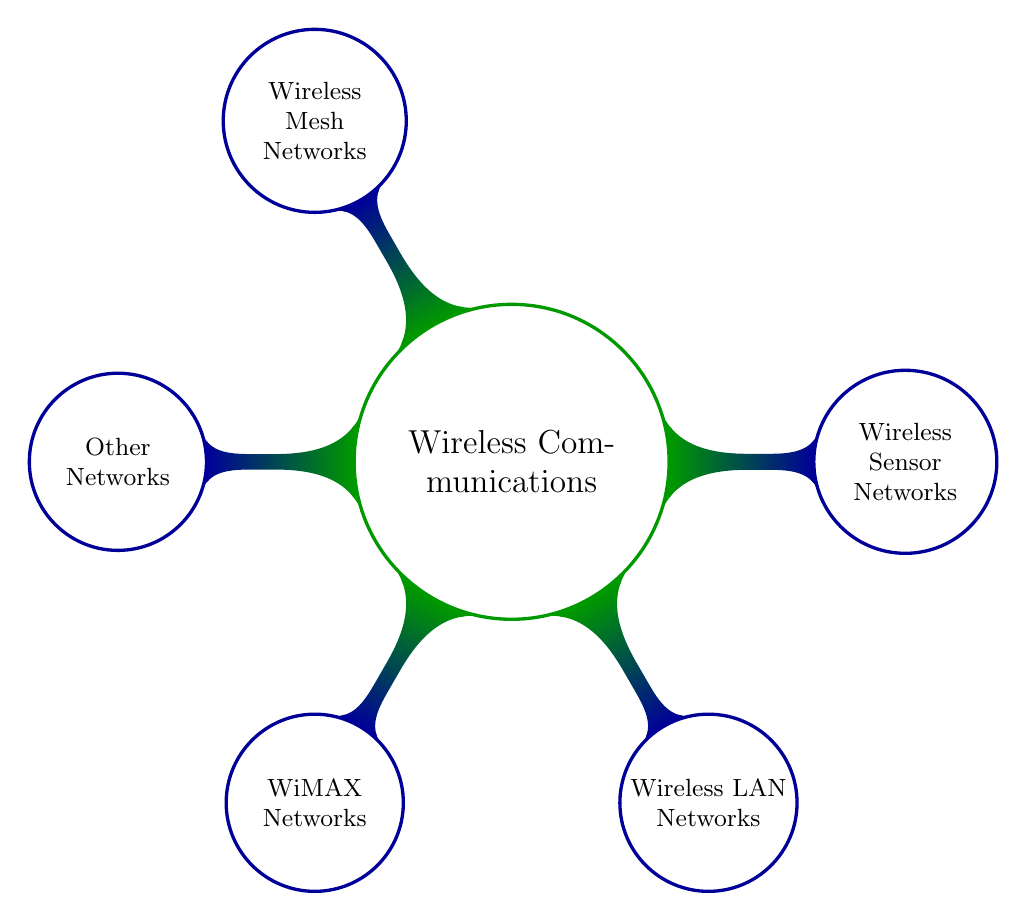
\begin{tikzpicture}
\centering
\usetikzlibrary{mindmap,trees}
\tikzset{concept/.append style={fill={none}}}
  \path[mindmap,concept color=black!40!green,text=black]
    node[concept] {Wireless Communications}
    [clockwise from=0]
    child[concept color=black!40!blue] { node[concept] {Wireless Sensor Networks} }
    child[concept color=black!40!blue] { node[concept] {Wireless LAN Networks} }
    child[concept color=black!40!blue] { node[concept] {WiMAX Networks} }
    child[concept color=black!40!blue] { node[concept] {Other Networks} }
    child[concept color=black!40!blue] { node[concept] {Wireless Mesh Networks} };
\end{tikzpicture}
}
\caption{Scope of the survey paper}
\label{fig:scope}
\end{center}
\end{figure*}



\begin{figure*}[!htb]
\begin{center}

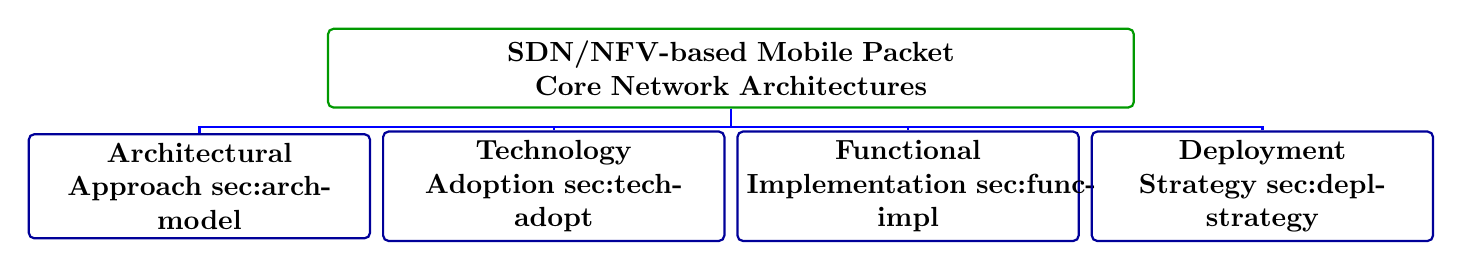
\begin{tikzpicture}[level 1/.style={sibling distance=45mm}]
% root of the the initial tree, level 1
  \node[root] {{\bf SDN/NFV-based Mobile Packet Core Network Architectures}}
[edge from parent fork down, draw = blue, thick]
% The first level, as children of the initial tree
    child {node[level 2] (c1) {{\bf Architectural \\ Approach~\autoref{sec:arch-model}}}}
    child {node[level 2] (c2) {{\bf Technology \\ Adoption~\autoref{sec:tech-adopt}}}}
    child {node[level 2] (c3) {{\bf Functional \\ Implementation~\autoref{sec:func-impl}}}}
    child {node[level 2] (c4) {{\bf Deployment \\ Strategy~\autoref{sec:depl-strategy}}}};
\end{tikzpicture}
\caption{Classification taxonomy tree with four dimensions: architectural approach, technology adoption, functional implementation, and deployment strategy}
\label{fig:taxonomy}
\end{center}
\end{figure*}
\bibliographystyle{ieeetr}
% argument is your BibTeX string definitions and bibliography database(s)
\bibliography{references}
\end{document}
